\setcounter{section}{2}
\section{Hàm số lượng giác}
\subsection{Tóm tắt lý thuyết}
\begin{tomtat}
	% \subsubsection{Định nghĩa hàm số lượng giác}
	% \begin{dn}
	% 	\begin{itemize}
	% 		\item Hàm số sin $y=\sin x$ có tập xác định là $\mathbb{R}$.
	% 		\item Hàm số cos $y=\cos x$ có tập xác định là $\mathbb{R}$.
	% 		\item Hàm số tan  $y=\tan x$ có tập xác định là $\mathbb{R} \setminus\left\{\dfrac{\pi}{2}+k \pi \Big| k \in \mathbb{Z} \right\}$.
	% 		\item  Hàm số cot $y=\cot x$ có tập xác định là $\mathbb{R} \setminus \left\{k \pi \Big| k \in \mathbb{Z} \right\}$.
	% 	\end{itemize}
	% \end{dn}
	\subsubsection{Hàm số chẵn, hàm số lẻ}
	\begin{dn}
	Cho hàm số $y=f(x)$ có tập xác định là $\mathscr{D}$.
	\begin{itemize}
		\item Hàm số $f(x)$ được gọi là \textbf{hàm số chẵn} nếu $\forall x \in \mathscr{D}$ thì $-x \in \mathscr{D}$ và $f(-x)=f(x)$. Đồ thị của một hàm số chẵn nhận trục tung là trục đối xứng.
		\item Hàm số $f(x)$ được gọi là \textbf{hàm số lẻ} nếu $\forall x \in \mathscr{D}$ thì $-x \in \mathscr{D}$ và $f(-x)=-f(x)$. Đồ thị của một hàm số lẻ nhận gốc toạ độ là tâm đối xứng.
	\end{itemize}
	\end{dn}
	\subsubsection{Hàm số tuần hoàn}
	\begin{dn}
		Hàm số $y=f(x)$ có tập xác định $\mathscr{D}$ được gọi là \textbf{hàm số tuần hoàn} nếu tồn tại số $T \neq 0$ sao cho với mọi $x \in \mathscr{D}$ ta có:
		\begin{enumerate}[i)]
			\item $x+T \in \mathscr{D}$ và $x-T \in \mathscr{D}$;
			\item $f(x+T)=f(x)$.
		\end{enumerate}
		Số $T$ dương nhỏ nhất thỏa mãn các điều kiện trên (nếu có) được gọi là \textbf{chu kì} của hàm số tuần hoàn đó.
	\end{dn}
	\begin{nx}
		\
		\begin{itemize}
			\item  Các hàm số $y=\sin x$ và $y=\cos x$ tuần hoàn với chu kì $2 \pi$. Các hàm số $y=\tan x$ và $y=\cot x$ tuần hoàn với chu kì $\pi$.
		\end{itemize}
	\end{nx}
	\begin{note} 
		Tổng quát, người ta chứng minh được các hàm số $y=A \sin \omega x$ và $y=A \cos \omega x$ $(\omega>0)$ là những hàm số tuần hoàn với chu kì \fbox{$T=\dfrac{2 \pi}{\omega}$}.
	\end{note}
	\subsubsection{Đồ thị và tính chất của hàm số $y=\sin x$}
	\begin{tc}
		Hàm số $y=\sin x$:
		\begin{itemize}
			\item   Có tập xác định là $\mathbb{R}$ và tập giá trị là $[-1 ; 1]$;
			\item   Là hàm số lẻ và tuần hoàn với chu kì $2 \pi$;
			\item    Đồng biến trên mỗi khoảng $\left(-\dfrac{\pi}{2}+k 2 \pi ; \dfrac{\pi}{2}+k 2 \pi\right)$ và nghịch biến trên mỗi khoảng \\
			$\left(\dfrac{\pi}{2}+k 2 \pi ; \dfrac{3 \pi}{2}+k 2 \pi\right)$, $k \in \mathbb{Z}$;
			\item    Có đồ thị đối xứng qua gốc toạ độ và gọi là một \textbf{đường hình sin}.
		\end{itemize}
	\begin{center}
		\begin{tikzpicture}[>=stealth,scale=0.7,transform shape] 
			\path
			({-2.5*pi},0) coordinate (X1)
			({-2*pi},0) coordinate (X2)
			({-1.5*pi},0) coordinate (X3)
			({-pi},0) coordinate (X4)
			({-0.5*pi},0) coordinate (X5)
			(0,0) coordinate (O)
			({0.5*pi},0) coordinate (X6)
			({pi},0) coordinate (X7)
			({1.5*pi},0) coordinate (X8)
			({2*pi},0) coordinate (X9)
			({2.5*pi},0) coordinate (X10)
			({-pi},-2) coordinate (A)
			({pi},-2) coordinate (B)
			;
			\draw[->] (-9.5,0) -- (9.5,0) node[below] {\small $x$};
			\draw[->] (0,-1.5) -- (0,1.8) node[right] {\small $y$};
			\draw [dotted] (X3)--({-1.5*pi},1)--({2.5*pi},1)--({2.5*pi},0)  ({0.5*pi},1)--({0.5*pi},0)
			(X1)--({-2.5*pi},-1)--({1.5*pi},-1)--({1.5*pi},0)  ({-0.5*pi},-1)--({-0.5*pi},0)
			({-pi},0) -- (A) ({pi},0) -- (B);
			\foreach \x/\g/\z in {X1/90/-\tfrac{5\pi}{2},X2/140/-2\pi,X3/-90/-\tfrac{3\pi}{2},X4/-135/-\pi,X5/90/-\tfrac{\pi}{2},X6/-90/\tfrac{\pi}{2},X7/60/\pi,X8/90/\tfrac{3\pi}{2},X9/-40/2\pi,X10/-90/\tfrac{5\pi}{2}} 
			\fill[black] (\x) circle(1pt) +(\g:5mm) node {$\z$};
			\draw [<->] ({-pi},-1.7)--({pi},-1.7) ; 
			\draw (0,0) node[below right]{$O$} (0,-1.7) node[below]{$T=2\pi$}
			(0,1) node[above right]{$1$} (0,-1) node[below right]{$-1$};
			\clip (-9.5,-1.4) rectangle (9.5,1.6) ;
			\draw[thick,samples=100,domain=-9.3:9.3] plot(\x,{sin((\x)*180/pi)});
			
		\end{tikzpicture}
	\end{center}
	\end{tc}
	\subsubsection{Đồ thị và tính chất của hàm số $y=\cos x$}
	\begin{tc}
		Hàm số $y=\cos x$:
		\begin{itemize}
			\item    Có tập xác định là $\mathbb{R}$ và tập giá trị là $[-1 ; 1]$;
			\item    Là hàm số chẵn và tuần hoàn với chu kì $2 \pi$;
			\item    Đồng biến trên mỗi khoảng $(-\pi+k 2 \pi ; k 2 \pi)$ và nghịch biến trên mỗi khoảng $(k 2 \pi ; \pi+k 2 \pi), k \in \mathbb{Z}$;
			\item    Có đồ thị là một đường hình sin đối xứng qua trục tung.
		\end{itemize}
	\begin{center}
		\begin{tikzpicture}[>=stealth,scale=0.77,transform shape] 
			\path
			({-2.5*pi},0) coordinate (X1)
			({-2*pi},0) coordinate (X2)
			({-1.5*pi},0) coordinate (X3)
			({-pi},0) coordinate (X4)
			({-0.5*pi},0) coordinate (X5)
			(0,0) coordinate (O)
			({0.5*pi},0) coordinate (X6)
			({pi},0) coordinate (X7)
			({1.5*pi},0) coordinate (X8)
			({2*pi},0) coordinate (X9)
			({2.5*pi},0) coordinate (X10)
			({-pi},-2) coordinate (A)
			({pi},-2) coordinate (B)
			;
			\draw[->] (-9.5,0) -- (9.5,0) node[below] {\small $x$};
			\draw[->] (0,-1.5) -- (0,1.8) node[right] {\small $y$};
			\draw [dotted] (X2)--({-2*pi},1)--({2*pi},1)--({2*pi},0) (X4)--({-pi},-1)--({pi},-1)--({pi},0) 
			({-pi},0) -- (A) ({pi},0) -- (B);
			\foreach \x/\g/\z in {X1/125/-\tfrac{5\pi}{2},X2/-90/-2\pi,X3/-120/-\tfrac{3\pi}{2},X4/90/-\pi,X5/110/-\tfrac{\pi}{2},X6/-120/\tfrac{\pi}{2},X7/90/\pi,X8/120/\tfrac{3\pi}{2},X9/-90/2\pi,X10/-120/\tfrac{5\pi}{2}} 
			\fill[black] (\x) circle(1pt) +(\g:5mm) node {$\z$};
			\draw [<->] ({-pi},-1.7)--({pi},-1.7) ; 
			\draw (0,0) node[below right]{$O$} (0,-1.7) node[below]{$T=2\pi$}
			(0,1) node[above right]{$1$} (0,-1) node[below right]{$-1$}
			;
			\clip (-9.5,-1.4) rectangle (9.5,1.6) ;
			\draw[thick,samples=100,domain=-9.3:9.3] plot(\x,{cos((\x)*180/pi)});
			
		\end{tikzpicture}
	\end{center}
	\end{tc}
	\subsubsection{Đồ thị và tính chất của hàm số $y=\tan x$}
	\begin{tc}
		Hàm số $y=\tan x$:
		\begin{itemize}
			\item    Có tập xác định là $\mathbb{R} \setminus\left\{\dfrac{\pi}{2}+k \pi \Big| k \in \mathbb{Z} \right\}$ và tập giá trị là $\mathbb{R}$;
			\item    Là hàm số lẻ và tuần hoàn với chu kì $\pi$;
			\item    Đồng biến trên mỗi khoảng $\left(-\dfrac{\pi}{2}+k \pi ; \dfrac{\pi}{2}+k \pi\right)$, $k \in \mathbb{Z}$;
			\item    Có đồ thị đối xứng qua gốc toạ độ.
		\end{itemize}
	\begin{center}
		\begin{tikzpicture}[>=stealth,scale=0.77,transform shape] 
			\path
			({-1.5*pi},0) coordinate (X1)
			({-pi},0) coordinate (X2)
			({-0.5*pi},0) coordinate (X3)
			({0.5*pi},0) coordinate (X4)
			({pi},0) coordinate (X5)
			({1.5*pi},0) coordinate (X6)
			;
			\draw[->] (-6.5,0) -- (6.5,0) node[below] {\small $x$};
			\draw[->] (0,-3.5) -- (0,3.5) node[right] {\small $y$};
			\draw [dashed] ({-3*pi/2},3.5)--({-3*pi/2},-3.5) ({-pi/2},3.5)--({-pi/2},-3.5) ({pi/2},3.5)--({pi/2},-3.5) ({3*pi/2},3.5)--({3*pi/2},-3.5) ;
			\foreach \x/\g/\z in {X1/-150/-\tfrac{3\pi}{2},X2/-40/-\pi,X3/-40/-\tfrac{\pi}{2},X4/-40/\tfrac{\pi}{2},X5/-400/\pi,X6/-40/\tfrac{3\pi}{2}} 
			\fill[black] (\x) circle(1pt) +(\g:5mm) node {$\z$};
			\draw (0,0) node[below right]{$O$};
			\clip (-6.5,-3.5) rectangle (6.5,3.5) ;
			\draw[thick,samples=100,domain={-pi/2+0.2}:{pi/2-0.2}] plot(\x,{tan((\x)*180/pi)});
			\draw[thick,samples=100,domain={pi/2+0.2}:{3*pi/2-0.2}] plot(\x,{tan((\x)*180/pi)});
			\draw[thick,samples=100,domain={-3*pi/2+0.2}:{-pi/2-0.2}] plot(\x,{tan((\x)*180/pi)});
		\end{tikzpicture}
	\end{center}
	\end{tc}
	\subsubsection{Đồ thị và tính chất của hàm số $y=\cot x$}
	\begin{tc}
		Hàm số $y=\cot x$:
		\begin{itemize}
			\item    Có tập xác định là $\mathbb{R} \setminus\{k \pi \mid k \in \mathbb{Z} \}$ và tập giá trị là $\mathbb{R}$; 
			\item    Là hàm số lẻ và tuần hoàn với chu kì $\pi$;
			\item    Nghịch biến trên mỗi khoảng $(k \pi ; \pi+k \pi), k \in \mathbb{Z}$;
			\item    Có đồ thị đối xứng qua gốc toạ độ.
		\end{itemize}
	\begin{center}
		\begin{tikzpicture}[>=stealth,scale=0.77,transform shape] 
			\path
			({-2*pi},0) coordinate (X1)
			({-1.5*pi},0) coordinate (X2)
			({-pi},0) coordinate (X3)
			({-0.5*pi},0) coordinate (X4)
			({0.5*pi},0) coordinate (X5)
			({pi},0) coordinate (X6)
			({1.5*pi},0) coordinate (X7)
			({2*pi},0) coordinate (X8)
			;
			\draw[->] (-7.5,0) -- (7.5,0) node[below] {\small $x$};
			\draw[->] (0,-3.5) -- (0,3.5) node[left] {\small $y$};
			\draw [dashed] ({-2*pi},3.5)--({-2*pi},-3.5) ({-pi},3.5)--({-pi},-3.5) ({pi},3.5)--({pi},-3.5) ({2*pi},3.5)--({2*pi},-3.5) ;
			\foreach \x/\g/\z in {X1/-150/-2\pi,X2/-130/-\tfrac{3\pi}{2},X3/-140/-\pi,X4/-100/-\tfrac{\pi}{2},X5/-100/\tfrac{\pi}{2},X6/-120/\pi,X7/-100/\tfrac{3\pi}{2}, X8/-120/2\pi}
			\fill[black] (\x) circle(1pt) +(\g:5mm) node {$\z$};
			\draw (0,0) node[below left]{$O$};
			\clip (-6.5,-3.5) rectangle (6.5,3.5) ;
			\draw[thick,samples=100,domain={0.2}:{pi-0.2}] plot(\x,{cot((\x)*180/pi)});
			\draw[thick,samples=100,domain={pi+0.2}:{2*pi-0.2}] plot(\x,{cot((\x)*180/pi)});
			\draw[thick,samples=100,domain={-0.2}:{-pi+0.2}] plot(\x,{cot((\x)*180/pi)});
			\draw[thick,samples=100,domain={-pi-0.2}:{-2*pi+0.2}] plot(\x,{cot((\x)*180/pi)});
		\end{tikzpicture}
	\end{center}
	\end{tc}
\end{tomtat}
\subsection{Các dạng toán thường gặp}
